% Options for packages loaded elsewhere
\PassOptionsToPackage{unicode}{hyperref}
\PassOptionsToPackage{hyphens}{url}
%
\documentclass[
  12pt,
]{article}
\usepackage{lmodern}
\usepackage{amssymb,amsmath}
\usepackage{ifxetex,ifluatex}
\ifnum 0\ifxetex 1\fi\ifluatex 1\fi=0 % if pdftex
  \usepackage[T1]{fontenc}
  \usepackage[utf8]{inputenc}
  \usepackage{textcomp} % provide euro and other symbols
\else % if luatex or xetex
  \usepackage{unicode-math}
  \defaultfontfeatures{Scale=MatchLowercase}
  \defaultfontfeatures[\rmfamily]{Ligatures=TeX,Scale=1}
  \setmainfont[]{Times New Roman}
\fi
% Use upquote if available, for straight quotes in verbatim environments
\IfFileExists{upquote.sty}{\usepackage{upquote}}{}
\IfFileExists{microtype.sty}{% use microtype if available
  \usepackage[]{microtype}
  \UseMicrotypeSet[protrusion]{basicmath} % disable protrusion for tt fonts
}{}
\makeatletter
\@ifundefined{KOMAClassName}{% if non-KOMA class
  \IfFileExists{parskip.sty}{%
    \usepackage{parskip}
  }{% else
    \setlength{\parindent}{0pt}
    \setlength{\parskip}{6pt plus 2pt minus 1pt}}
}{% if KOMA class
  \KOMAoptions{parskip=half}}
\makeatother
\usepackage{xcolor}
\IfFileExists{xurl.sty}{\usepackage{xurl}}{} % add URL line breaks if available
\IfFileExists{bookmark.sty}{\usepackage{bookmark}}{\usepackage{hyperref}}
\hypersetup{
  pdftitle={Community Ecology in Coweeta Long Term Ecological Research},
  pdfauthor={Michael Gaffney, Eni Bihari, \& Cal Oakley},
  hidelinks,
  pdfcreator={LaTeX via pandoc}}
\urlstyle{same} % disable monospaced font for URLs
\usepackage[margin=2.54cm]{geometry}
\usepackage{longtable,booktabs}
% Correct order of tables after \paragraph or \subparagraph
\usepackage{etoolbox}
\makeatletter
\patchcmd\longtable{\par}{\if@noskipsec\mbox{}\fi\par}{}{}
\makeatother
% Allow footnotes in longtable head/foot
\IfFileExists{footnotehyper.sty}{\usepackage{footnotehyper}}{\usepackage{footnote}}
\makesavenoteenv{longtable}
\usepackage{graphicx,grffile}
\makeatletter
\def\maxwidth{\ifdim\Gin@nat@width>\linewidth\linewidth\else\Gin@nat@width\fi}
\def\maxheight{\ifdim\Gin@nat@height>\textheight\textheight\else\Gin@nat@height\fi}
\makeatother
% Scale images if necessary, so that they will not overflow the page
% margins by default, and it is still possible to overwrite the defaults
% using explicit options in \includegraphics[width, height, ...]{}
\setkeys{Gin}{width=\maxwidth,height=\maxheight,keepaspectratio}
% Set default figure placement to htbp
\makeatletter
\def\fps@figure{htbp}
\makeatother
\setlength{\emergencystretch}{3em} % prevent overfull lines
\providecommand{\tightlist}{%
  \setlength{\itemsep}{0pt}\setlength{\parskip}{0pt}}
\setcounter{secnumdepth}{5}

\title{Community Ecology in Coweeta Long Term Ecological Research}
\usepackage{etoolbox}
\makeatletter
\providecommand{\subtitle}[1]{% add subtitle to \maketitle
  \apptocmd{\@title}{\par {\large #1 \par}}{}{}
}
\makeatother
\subtitle{\url{https://github.com/mtgaffney/BihariGaffneyOakley_ENV872_EDA_FinalProject.git}}
\author{Michael Gaffney, Eni Bihari, \& Cal Oakley}
\date{}

\begin{document}
\maketitle

\newpage
\tableofcontents 
\newpage
\listoftables 
\newpage
\listoffigures 
\newpage

\hypertarget{rationale-and-research-questions}{%
\section{Rationale and Research
Questions}\label{rationale-and-research-questions}}

Coweeta Long Term Ecological Research (LTER) is one of the oldest long
term ecological research sites in the United States. It's located in the
eastern deciduous forest of the southern Appalachian Mountains,
specifically Macon County, North Carolina. This ecosystem is
ecologically valuable because of its combination of old age, high
productivity, temperate biodiversity, \& high environmental variation
(NSF 2018). These last two factors are the ones on which our
investigation will focus.

The southern Appalachians are home to numerous woody plant species.
These species each have unique characteristics that make them better
suited for certain sites more than others (think of shade tolerance,
drought tolerance, or nutrient requirements). Also, the southern
Appalachian mountains are so topographically diverse that species with
vastly different site requirements can often be found within close
proximity to one another, while groups of the same species are found far
apart. This presents a challenge to researchers interested in community
ecology because unless you collect extensive environmental measurements
at every research site they cannot understand why a species assemblages
occurs where it does. That is why we want to perform a comprehensive
analysis of environmental and species occurrence data to determine if
there are more general environmental trends that can explain the
distribution of woody species at Coweeta.

\newpage

\hypertarget{dataset-information}{%
\section{Dataset Information}\label{dataset-information}}

Three datasets in total were used for this analysis, all provided by
Urban. Species data consists the basal area (BA) of 18 species across
108 plots in Coweeta. Environmental data consists of 20 environmental
variables across the same 108 sites. Finally, we were provided
geospatial data for the sites.

\begin{longtable}[]{@{}lll@{}}
\toprule
Species Code & Scientific Name & Common Name\tabularnewline
\midrule
\endhead
ACRU & Acer rubrum & Red Maple\tabularnewline
AMAR & Amelanchier arborea & Common Serviceberry\tabularnewline
BELE & Betula lenta & Sweet Birch\tabularnewline
CAGL & Carya glabra & Pignut Hickory\tabularnewline
CATO & Carya tomentosa & Mockernut Hickory\tabularnewline
COFL & Cornus florida & Flowering Dogwood\tabularnewline
KALA & Kalmia latifolia & Mountain Laurel\tabularnewline
LITU & Liriodendron tulipifera & Tulip Tree\tabularnewline
NYSY & Nyssa sylvatica & Black Tupelo\tabularnewline
OXAR & Oxydendron arboreum & Sourwood\tabularnewline
PIRI & Pinus rigida & Pitch Pine\tabularnewline
QUAL & Quercus alba & White Oak\tabularnewline
QUCO & Quercus coccinea & Scarlet Oak\tabularnewline
QUPR & Quercus prinus & Chestnut Oak\tabularnewline
QURU & Quercus rubra & Red Oak\tabularnewline
QUVE & Quercus velutina & Black Oak\tabularnewline
RHMA & Rhododendron maximum & Great Laurel\tabularnewline
ROPS & Robinia pseudoacacia & Black Locust\tabularnewline
\bottomrule
\end{longtable}

\begin{longtable}[]{@{}ll@{}}
\toprule
Variable & Description\tabularnewline
\midrule
\endhead
Elevation & Elevation (M)\tabularnewline
SlopeDEM & Slope\tabularnewline
TAspectD & Transformed Aspect\tabularnewline
TCI & Topograhpic Convergence Index\tabularnewline
xDepth & Mean soil depth (cm)\tabularnewline
sDepth & Standard deviation of depth\tabularnewline
pH & pH\tabularnewline
Acidity & Acidity\tabularnewline
Ca & Calcium (cmol(+)/kg)\tabularnewline
K & Potassium (cmol(+)/kg)\tabularnewline
Mg & Magnesium (cmol(+)/kg)\tabularnewline
P & Phosphorous (g/g)\tabularnewline
C & Soil carbon (\%)\tabularnewline
N & Nitrogen (\%)\tabularnewline
C:N & Carbon:Nitrogen ratio\tabularnewline
ECEC & Effective Cation Exchange Capacity\tabularnewline
BS & Base Saturation\tabularnewline
Clay & Clay (\%)\tabularnewline
Silt & Silt (\%)\tabularnewline
Sand & Sand (\%)\tabularnewline
\bottomrule
\end{longtable}

\begin{figure}
\centering
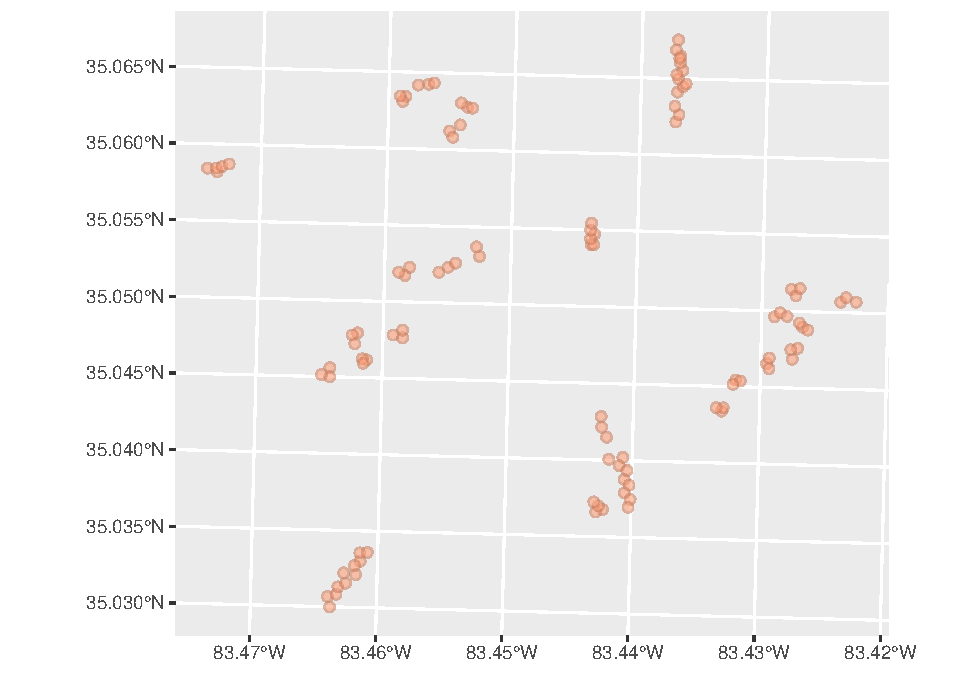
\includegraphics{ProjectDraft_files/figure-latex/unnamed-chunk-1-1.pdf}
\caption{Geographic distribution of the 108 Coweeta plots.}
\end{figure}

\newpage

\hypertarget{exploratory-analysis}{%
\section{Exploratory Analysis}\label{exploratory-analysis}}

We first explored the species composition of the Coweeta plots by
looking at the mean basal area (BA) per species. We did this separately
for the canopy and understory species, since these species play very
different ecological roles in these ecosystems. The canopy and
understory are made up of very different species, and the trees have
very different sizes and abundances. Canopy trees tend to be sparser and
larger, while understory trees tend to be denser and smaller. Chestnut
oak (QUPR), red maple (ACRU), northern red oak (QURU), and scarlet oak
(QUCO) are the trees that make up the most BA among overstory trees,
which is to be expected in these oak-hickory dominated mountainous
ecosystems. The highest BA understory species is a native rhododendron
(RHMA), which is also to be expected in these ecosystems.

\begin{figure}
\centering
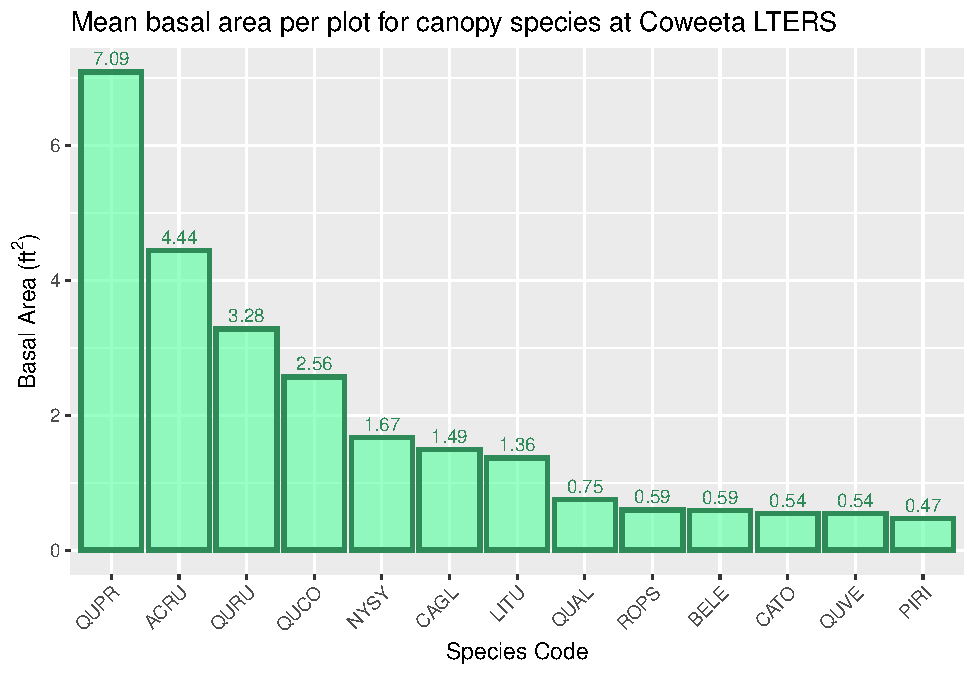
\includegraphics{ProjectDraft_files/figure-latex/unnamed-chunk-2-1.pdf}
\caption{Mean basal area per plot for canopy species at Coweeta LTERS.}
\end{figure}

\begin{figure}
\centering
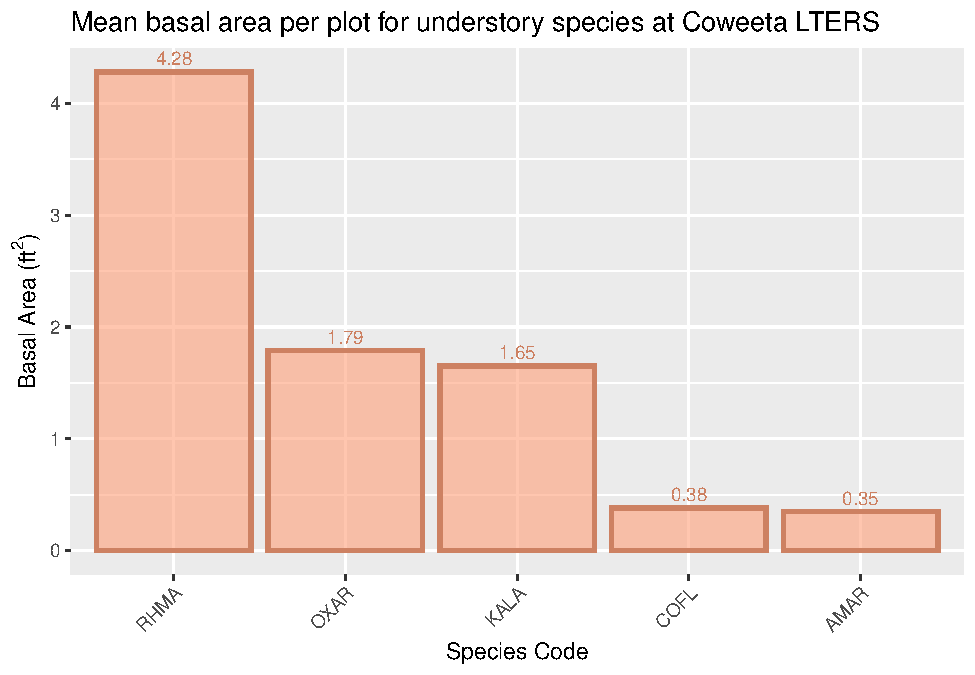
\includegraphics{ProjectDraft_files/figure-latex/unnamed-chunk-3-1.pdf}
\caption{Mean basal area per plot for understory species at Coweeta
LTERS.}
\end{figure}

We also explored the basal area distributions individually for some of
the most common canopy species in Coweeta. These distributions are
sharply skewed right for all 4 species, which can be expected for the
dominant trees in such ecosystems. This simply means that there are very
many small trees and very few large trees, which makes sense based on
their reproductive strategy. These trees produce a lot of seeds and
stump sprouts, but only a fraction of these survive into old age.

We also created a cowplot of all of these species alongside one another
for easy comparison.

\begin{figure}
\centering
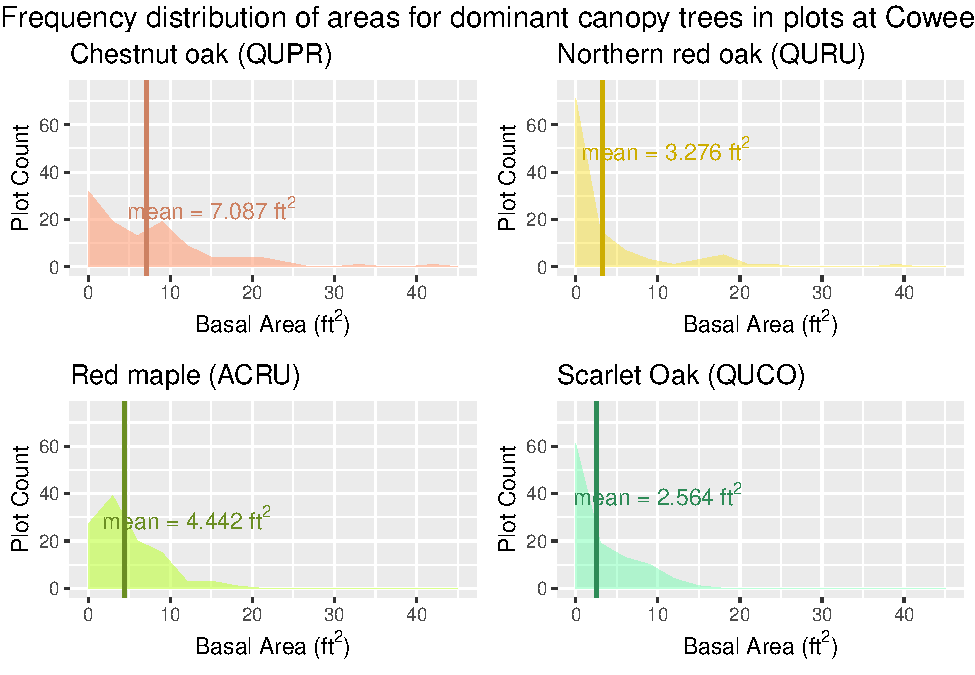
\includegraphics{ProjectDraft_files/figure-latex/unnamed-chunk-5-1.pdf}
\caption{Frequency distribution of areas for dominant canopy trees in
plots at Coweeta LTRS.}
\end{figure}

Finally, explored some of the environmetnal variables. Although our
method of analysis for this data set will not require us to eliminate
correlated variables for statistical purposes, it is worth exploring
what some of the correlations are.

\newpage

\hypertarget{analysis}{%
\section{Analysis}\label{analysis}}

\textbf{Question:}

Our question for this analysis is: what environmental variables, or
complex of variables, primarily sorts tree communities in Coweeta? Our
initial hypothesis, following a similiar study conducted by Urban et
al.~(2000), is that elevation, serving as a proxy for both temperature
and moisture, will function as the primary sorting mechanism for tree
species. In order to answer this question, we elected to use Nonmetric
Multidimensional Scaling (NMS). NMS is an ordination technique that can
visualize trends in complex, non-parametric, multivariate datasets. As a
technique, NMS simplifies complex data by plotting sites in ordination
space. The aim is to draw sites close together on a graph that are close
together ecologically. It converts ecological distance, in other words,
to graph distance.

NMS works through an iterative process. It creates a series of numerical
approximations that capture trends within the data. The process first
randomly scatters the plots, regresses the ordination distances and
ecological distances between the points, and then ``jitters'' the data
once again to create an improved configuration. A successful ordination
will create an ordination where ecological distance should correspond
with a 1:1 ratio with ordination distance; far ecological distance
should be far ordination distance.

NMS is particularly appropriate for this dataset because, unlike other
statistical tests, it makes no parametric assumptions about input data
sources; as tree basal are not normally distributed, this is
particularly advantageous. Additionally, NMS works particularly well
when there are a great deal of zeroes in the data, which is often the
case for species data on tree plots.

The NMS process began by screenign the environmetnal variables for
correlations and removing the correlated variables. Although the actual
NMS analysis was run on the species data, removing correlations is
important for visual purposes later on. We then relativized the original
species data to account for the vast difference in basal area between
some of the species. With this relativized data, we then created a
distance matrix from the species data. This is done using the ecodist
package, using the Bray Curtis method (Urban et al.~2007. This produces
a matrix that details how far apart each plot is ecologically from one
another. In other words, plots that are ecologically very
similar---having similar tree communities, species richness, and basal
area---will have different scores than those that are very far apart.

The next step in running the NMS was to start a stepdown procedure. This
involved producing a full 6 dimensional NMS object, and then evaluating
how well it performed. An NMS will produce two important values: and
R\textsuperscript{2} and stress values. With a full ordination, we
plotted these values to explore what the optimal number of dimensions
for the final NMS would be. The optimal number captures a significant
portion of the variance but also has low stress. In this case, 2 axes
appears to be the best configuration (with a stress value below .3 and
an R\textsuperscript{2} around .6).

\begin{verbatim}
## $names
## [1] "conf"   "stress" "r2"     "mindim" "maxdim" "nits"  
## 
## $class
## [1] "nmds"
\end{verbatim}

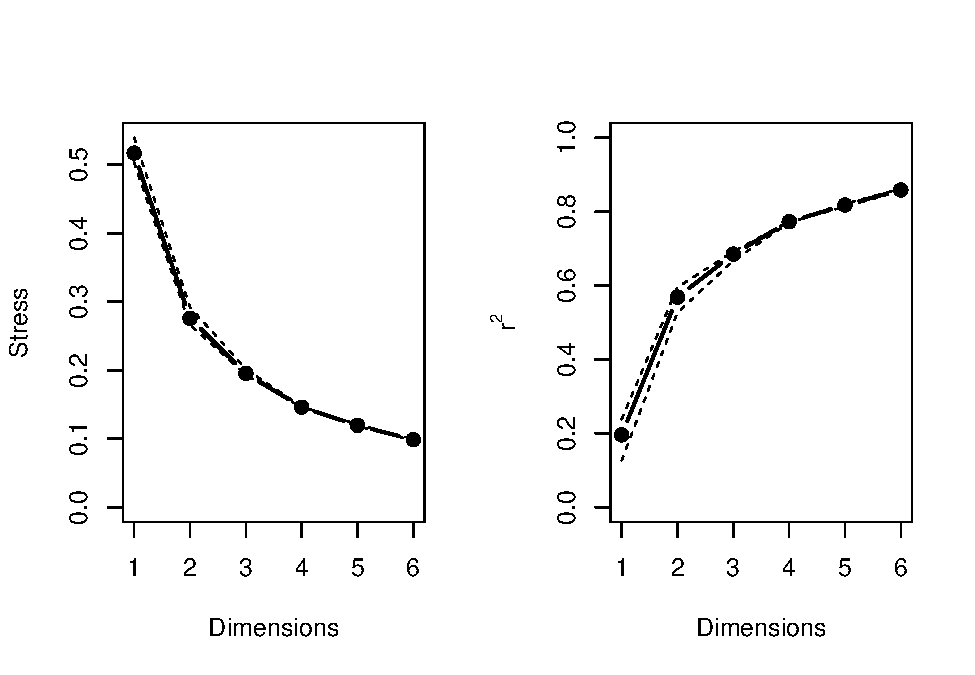
\includegraphics{ProjectDraft_files/figure-latex/unnamed-chunk-8-1.pdf}

We then ran a second final NMS with two dimensions. In this case, we
have R generate not one but twenty versions of this same NMS, so that we
can choose the one that performs best.

The final NMS object, however, is not directly intelligible. This is
because NMS generates all of the axes at the same time; in doing so, it
does not pay attention to importance. In practice, this means that in
order to properly understand what the axes are, it is necessary to run a
Principle Component Analysis (PCA) on the axes. The PCA effectively
rotates the initial NMS ordination in such a way so as to force the
points to align with the axes. It also makes axis 1 contain the majority
of the variance.

After rotating the NMS, we checked for how well the analysis performed.
We plotted a Shepard Diagram, which illustrates the relationship between
ecological distance and ordination distance. Ideally, this is a one to
one relationship; here, we see that the origination performed relatively
well in aligning ecological distance with ordination space. Here, we
also checked the overall R\textsuperscript{2} for the NMS, which was
roughly 60\% depending on the different runs. Of the variance explained,
roughly 36\% was captured by NMS 1, and the other 24\% was captured by
NMS 2.

\begin{figure}
\centering
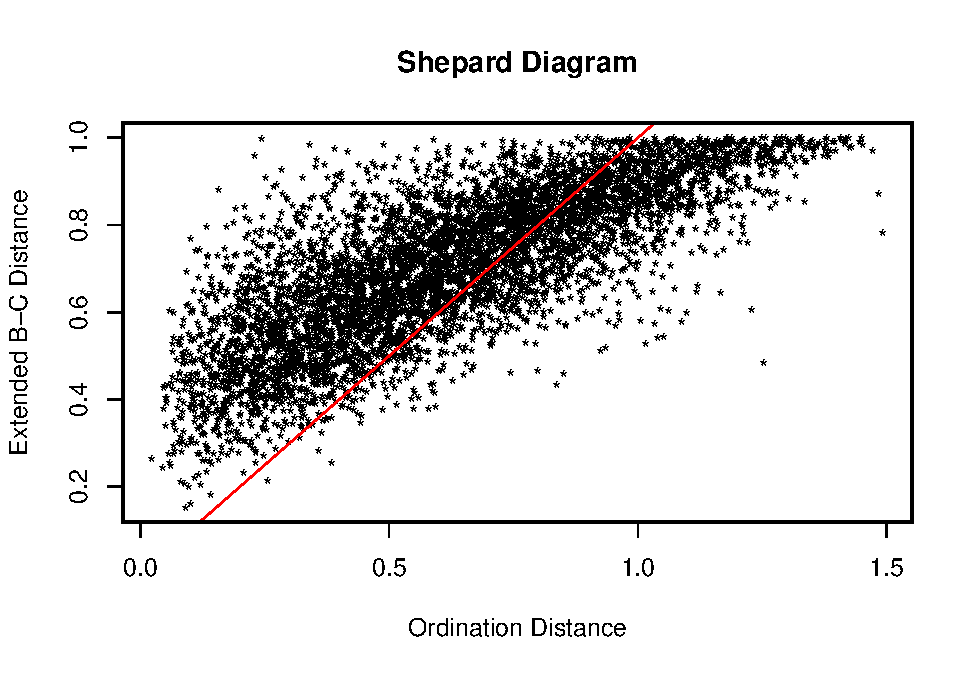
\includegraphics{ProjectDraft_files/figure-latex/unnamed-chunk-11-1.pdf}
\caption{Shepard Diagram showing the relationship between ordination
distance and ecological distance.}
\end{figure}

In order to fully understand the ecological implications of the
ordination we then created three different plots. We began by preparing
the data to be plotted with the ggplot package.

Then we created the plots. Figure 1 below shows a graph of the 108
Coweeta plots in ordination space. The first NMS axes (with most of the
variance) is on the y-axis, the second (with the rest of the variance)
is on the X axis. Placed on top of this ordination are correlation
vectors for all of the environmental variables. Effectively, they show
how well correlated the environmental variables are with the ordination
axes that were generated from the species data: the direction of the
vector shows the direction of the correlation (positive/negative), and
the length shows how strong the correlation is. Here, the C:N ratio is
strongly correlated with the first NMS axis, where K (potassium) is
negatively correlated. This suggests that NMS 1 likely represents a
gradient of soil properties, or, given the Coweeta system, it likely
represents a gradient of soil moisture. While NMS 2 contained far less
variance, it appears to be positively correlated with elevation, meaning
that it likely represents a rough elevation gradient.

\begin{figure}
\centering
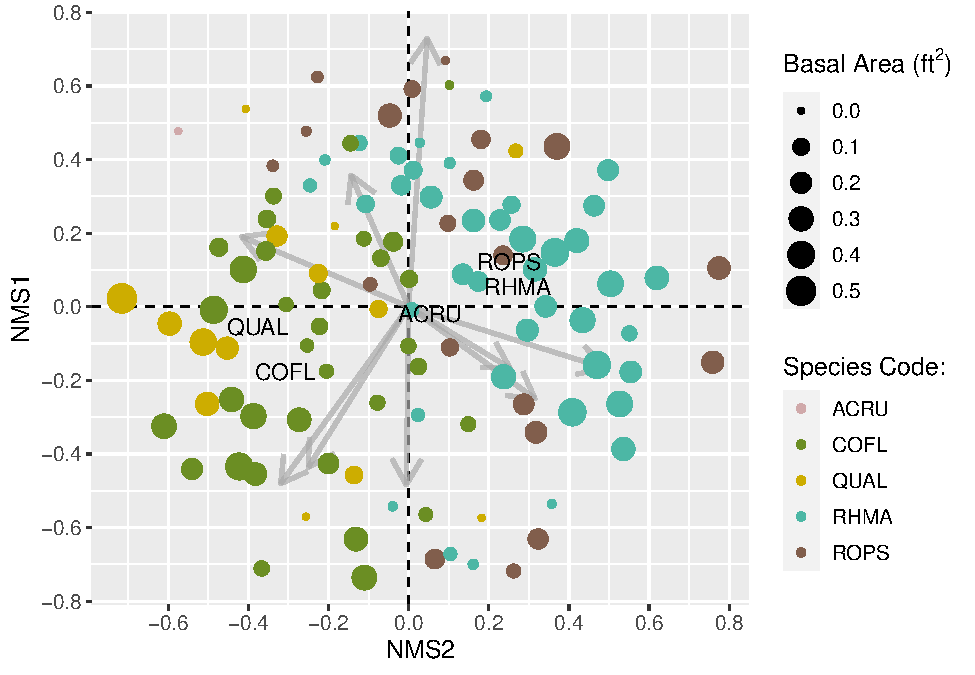
\includegraphics{ProjectDraft_files/figure-latex/unnamed-chunk-14-1.pdf}
\caption{Environmental vectors showing correlations in NMS space.}
\end{figure}

We further explored the meaning of the gradients by plotting individual
tree species by relative basal area into NMS space. Figure 2 below shows
6 species in ordination space sorted by the soil moisture gradient. What
is particularly evident here is the way that sweet birch (BELE) and
tulip trees (LITU) appear in the areas of relatively high soil moisture,
where pitch pine (PIRI), scarlet oak (QUCO) and mountain laurel tend to
appear in places with drier soils. Red maple (ACRU), a generalist,
appears all over and does not seem to favor any particular soil type.

\begin{figure}
\centering
\includegraphics{ProjectDraft_files/figure-latex/unnamed-chunk-15-1.pdf}
\caption{Tree species plotted in NMS space to illustrate sorting along
the soil moisture gradient (roughly NMS1).}
\end{figure}

Figure 3 emphasizes speices that sorted particular well on the elevation
gradient. White oak (QUAL) appears with flowering dogwood (COFL) more
often in lower elevation sites, where great laurel (RHMA) and black
locust (ROPS) appear at much higher elevations.

\begin{figure}
\centering
\includegraphics{ProjectDraft_files/figure-latex/unnamed-chunk-16-1.pdf}
\caption{Tree species plotted in NMS space to illustrate sorting along
the elevation gradient (roughly NMS2).}
\end{figure}

\newpage

\hypertarget{summary-and-conclusions}{%
\section{Summary and Conclusions}\label{summary-and-conclusions}}

Overall, these results suggest that in the Coweeta system, soil moisture
and composition plays a substantially stronger role in sorting species
than elevation does. The relatively light elevation gradient in the
southern Appalachians (compared to the profound gradient in the Sierran
system as Urban et al.~studied, for example), clearly affects the
pattern of different trees, but not as substantially as soil. With data
of environmetnal variables more attuned specifcally to soil moisture, it
might be possible to verify more specifically that thsi factor is what
sorts tree species in this space.

\newpage

\hypertarget{references}{%
\section{References}\label{references}}

Goslee, S.C. and Urban, D.L. 2007. The ecodist package for
dissimilarity-based analysis of ecological data. Journal of Statistical
Software 22(7):1-19.

Jari Oksanen, F. Guillaume Blanchet, Michael Friendly, Roeland Kindt,
Pierre Legendre, Dan McGlinn, Peter R. Minchin, R. B. O'Hara, Gavin L.
Simpson, Peter Solymos, M. Henry H. Stevens, Eduard Szoecs and Helene
Wagner (2020). vegan: Community Ecology Package. R package version
2.5-7. \url{https://CRAN.R-project.org/package=vegan}

Maechler, M., Rousseeuw, P., Struyf, A., Hubert, M., Hornik, K.(2021).
Cluster: Cluster Analysis Basics and Extensions. R package version
2.1.2.

R Core Team (2020). R: A language and environment for statistical
computing. R Foundation for Statistical Computing, Vienna, Austria. URL
\url{https://www.R-project.org/}.

Urban, D. L., Miller, C., Halpin, P. N., \& Stephenson, N. L. (2000).
Forest gradient response in Sierran landscapes: the physical template.
Landscape Ecology, 15(7), 603-620

\end{document}
